%\documentclass{standalone}
%\usepackage{tikz}
%\usetikzlibrary{patterns,plotmarks}
%\begin{document}
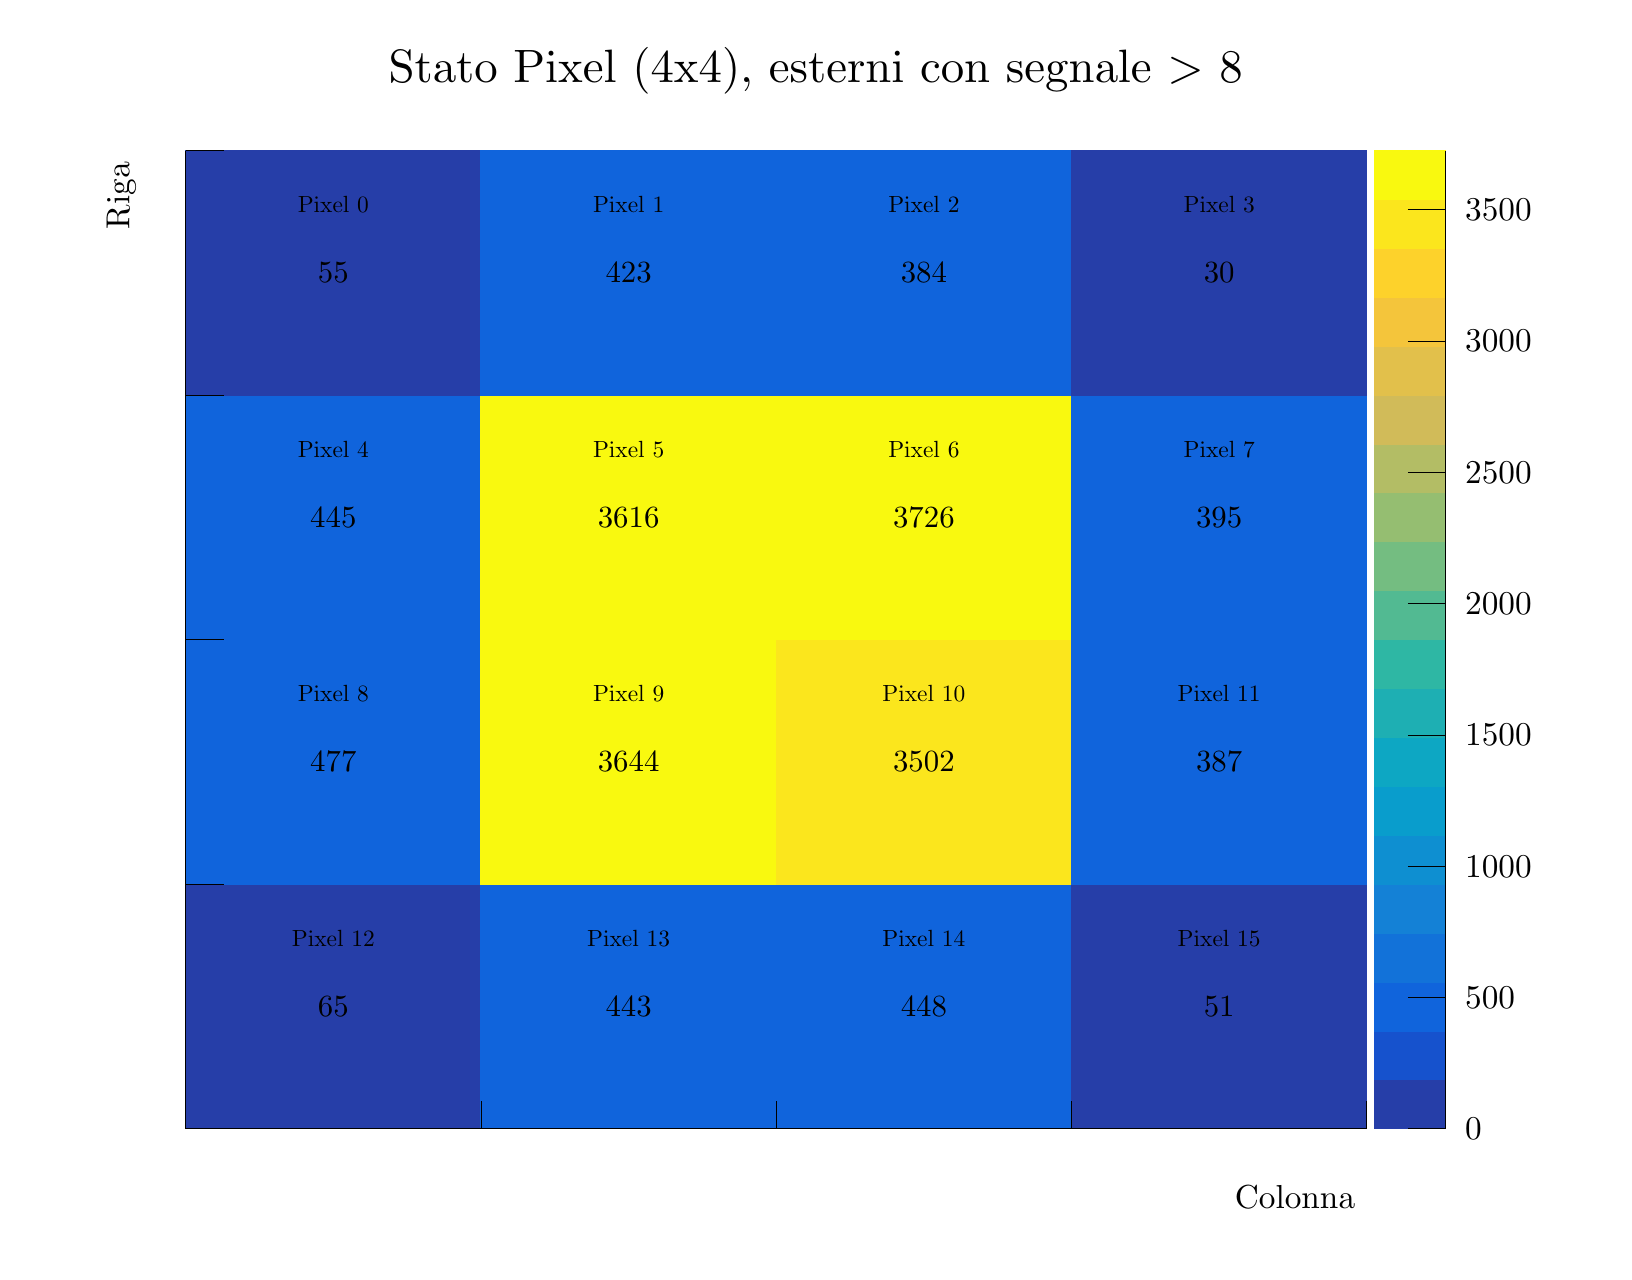
\begin{tikzpicture}
\def\CheckTikzLibraryLoaded#1{ \ifcsname tikz@library@#1@loaded\endcsname \else \PackageWarning{tikz}{usetikzlibrary{#1} is missing in the preamble.} \fi }
\CheckTikzLibraryLoaded{patterns}
\CheckTikzLibraryLoaded{plotmarks}
\pgfdeclareplotmark{cross} {
\pgfpathmoveto{\pgfpoint{-0.3\pgfplotmarksize}{\pgfplotmarksize}}
\pgfpathlineto{\pgfpoint{+0.3\pgfplotmarksize}{\pgfplotmarksize}}
\pgfpathlineto{\pgfpoint{+0.3\pgfplotmarksize}{0.3\pgfplotmarksize}}
\pgfpathlineto{\pgfpoint{+1\pgfplotmarksize}{0.3\pgfplotmarksize}}
\pgfpathlineto{\pgfpoint{+1\pgfplotmarksize}{-0.3\pgfplotmarksize}}
\pgfpathlineto{\pgfpoint{+0.3\pgfplotmarksize}{-0.3\pgfplotmarksize}}
\pgfpathlineto{\pgfpoint{+0.3\pgfplotmarksize}{-1.\pgfplotmarksize}}
\pgfpathlineto{\pgfpoint{-0.3\pgfplotmarksize}{-1.\pgfplotmarksize}}
\pgfpathlineto{\pgfpoint{-0.3\pgfplotmarksize}{-0.3\pgfplotmarksize}}
\pgfpathlineto{\pgfpoint{-1.\pgfplotmarksize}{-0.3\pgfplotmarksize}}
\pgfpathlineto{\pgfpoint{-1.\pgfplotmarksize}{0.3\pgfplotmarksize}}
\pgfpathlineto{\pgfpoint{-0.3\pgfplotmarksize}{0.3\pgfplotmarksize}}
\pgfpathclose
\pgfusepathqstroke
}
\pgfdeclareplotmark{cross*} {
\pgfpathmoveto{\pgfpoint{-0.3\pgfplotmarksize}{\pgfplotmarksize}}
\pgfpathlineto{\pgfpoint{+0.3\pgfplotmarksize}{\pgfplotmarksize}}
\pgfpathlineto{\pgfpoint{+0.3\pgfplotmarksize}{0.3\pgfplotmarksize}}
\pgfpathlineto{\pgfpoint{+1\pgfplotmarksize}{0.3\pgfplotmarksize}}
\pgfpathlineto{\pgfpoint{+1\pgfplotmarksize}{-0.3\pgfplotmarksize}}
\pgfpathlineto{\pgfpoint{+0.3\pgfplotmarksize}{-0.3\pgfplotmarksize}}
\pgfpathlineto{\pgfpoint{+0.3\pgfplotmarksize}{-1.\pgfplotmarksize}}
\pgfpathlineto{\pgfpoint{-0.3\pgfplotmarksize}{-1.\pgfplotmarksize}}
\pgfpathlineto{\pgfpoint{-0.3\pgfplotmarksize}{-0.3\pgfplotmarksize}}
\pgfpathlineto{\pgfpoint{-1.\pgfplotmarksize}{-0.3\pgfplotmarksize}}
\pgfpathlineto{\pgfpoint{-1.\pgfplotmarksize}{0.3\pgfplotmarksize}}
\pgfpathlineto{\pgfpoint{-0.3\pgfplotmarksize}{0.3\pgfplotmarksize}}
\pgfpathclose
\pgfusepathqfillstroke
}
\pgfdeclareplotmark{newstar} {
\pgfpathmoveto{\pgfqpoint{0pt}{\pgfplotmarksize}}
\pgfpathlineto{\pgfqpointpolar{44}{0.5\pgfplotmarksize}}
\pgfpathlineto{\pgfqpointpolar{18}{\pgfplotmarksize}}
\pgfpathlineto{\pgfqpointpolar{-20}{0.5\pgfplotmarksize}}
\pgfpathlineto{\pgfqpointpolar{-54}{\pgfplotmarksize}}
\pgfpathlineto{\pgfqpointpolar{-90}{0.5\pgfplotmarksize}}
\pgfpathlineto{\pgfqpointpolar{234}{\pgfplotmarksize}}
\pgfpathlineto{\pgfqpointpolar{198}{0.5\pgfplotmarksize}}
\pgfpathlineto{\pgfqpointpolar{162}{\pgfplotmarksize}}
\pgfpathlineto{\pgfqpointpolar{134}{0.5\pgfplotmarksize}}
\pgfpathclose
\pgfusepathqstroke
}
\pgfdeclareplotmark{newstar*} {
\pgfpathmoveto{\pgfqpoint{0pt}{\pgfplotmarksize}}
\pgfpathlineto{\pgfqpointpolar{44}{0.5\pgfplotmarksize}}
\pgfpathlineto{\pgfqpointpolar{18}{\pgfplotmarksize}}
\pgfpathlineto{\pgfqpointpolar{-20}{0.5\pgfplotmarksize}}
\pgfpathlineto{\pgfqpointpolar{-54}{\pgfplotmarksize}}
\pgfpathlineto{\pgfqpointpolar{-90}{0.5\pgfplotmarksize}}
\pgfpathlineto{\pgfqpointpolar{234}{\pgfplotmarksize}}
\pgfpathlineto{\pgfqpointpolar{198}{0.5\pgfplotmarksize}}
\pgfpathlineto{\pgfqpointpolar{162}{\pgfplotmarksize}}
\pgfpathlineto{\pgfqpointpolar{134}{0.5\pgfplotmarksize}}
\pgfpathclose
\pgfusepathqfillstroke
}
\definecolor{c}{rgb}{1,1,1};
\draw [color=c, fill=c] (0,0) rectangle (20,15.5311);
\draw [color=c, fill=c] (2,1.55311) rectangle (17,13.978);
\definecolor{c}{rgb}{0,0,0};
\draw [c,line width=0.3] (2,1.55311) -- (2,13.978) -- (17,13.978) -- (17,1.55311) -- (2,1.55311);
\definecolor{c}{rgb}{1,1,1};
\draw [color=c, fill=c] (2,1.55311) rectangle (17,13.978);
\definecolor{c}{rgb}{0,0,0};
\draw [c,line width=0.3] (2,1.55311) -- (2,13.978) -- (17,13.978) -- (17,1.55311) -- (2,1.55311);
\definecolor{c}{rgb}{0.150523,0.241303,0.660565};
\draw [color=c, fill=c] (2,1.55311) rectangle (5.75,4.65932);
\definecolor{c}{rgb}{0.0633125,0.391444,0.861859};
\draw [color=c, fill=c] (5.75,1.55311) rectangle (9.5,4.65932);
\draw [color=c, fill=c] (9.5,1.55311) rectangle (13.25,4.65932);
\definecolor{c}{rgb}{0.150523,0.241303,0.660565};
\draw [color=c, fill=c] (13.25,1.55311) rectangle (17,4.65932);
\definecolor{c}{rgb}{0.0633125,0.391444,0.861859};
\draw [color=c, fill=c] (2,4.65932) rectangle (5.75,7.76553);
\definecolor{c}{rgb}{0.977,0.977044,0.0583656};
\draw [color=c, fill=c] (5.75,4.65932) rectangle (9.5,7.76553);
\definecolor{c}{rgb}{0.9842,0.903169,0.111953};
\draw [color=c, fill=c] (9.5,4.65932) rectangle (13.25,7.76553);
\definecolor{c}{rgb}{0.0633125,0.391444,0.861859};
\draw [color=c, fill=c] (13.25,4.65932) rectangle (17,7.76553);
\draw [color=c, fill=c] (2,7.76553) rectangle (5.75,10.8717);
\definecolor{c}{rgb}{0.977,0.977044,0.0583656};
\draw [color=c, fill=c] (5.75,7.76553) rectangle (9.5,10.8717);
\draw [color=c, fill=c] (9.5,7.76553) rectangle (13.25,10.8717);
\definecolor{c}{rgb}{0.0633125,0.391444,0.861859};
\draw [color=c, fill=c] (13.25,7.76553) rectangle (17,10.8717);
\definecolor{c}{rgb}{0.150523,0.241303,0.660565};
\draw [color=c, fill=c] (2,10.8717) rectangle (5.75,13.978);
\definecolor{c}{rgb}{0.0633125,0.391444,0.861859};
\draw [color=c, fill=c] (5.75,10.8717) rectangle (9.5,13.978);
\draw [color=c, fill=c] (9.5,10.8717) rectangle (13.25,13.978);
\definecolor{c}{rgb}{0.150523,0.241303,0.660565};
\draw [color=c, fill=c] (13.25,10.8717) rectangle (17,13.978);
\definecolor{c}{rgb}{0,0,0};
\draw (3.875,3.10621) node[scale=1.11271, color=c, rotate=0]{65};
\draw (7.625,3.10621) node[scale=1.11271, color=c, rotate=0]{443};
\draw (11.375,3.10621) node[scale=1.11271, color=c, rotate=0]{448};
\draw (15.125,3.10621) node[scale=1.11271, color=c, rotate=0]{51};
\draw (3.875,6.21242) node[scale=1.11271, color=c, rotate=0]{477};
\draw (7.625,6.21242) node[scale=1.11271, color=c, rotate=0]{3644};
\draw (11.375,6.21242) node[scale=1.11271, color=c, rotate=0]{3502};
\draw (15.125,6.21242) node[scale=1.11271, color=c, rotate=0]{387};
\draw (3.875,9.31864) node[scale=1.11271, color=c, rotate=0]{445};
\draw (7.625,9.31864) node[scale=1.11271, color=c, rotate=0]{3616};
\draw (11.375,9.31864) node[scale=1.11271, color=c, rotate=0]{3726};
\draw (15.125,9.31864) node[scale=1.11271, color=c, rotate=0]{395};
\draw (3.875,12.4248) node[scale=1.11271, color=c, rotate=0]{55};
\draw (7.625,12.4248) node[scale=1.11271, color=c, rotate=0]{423};
\draw (11.375,12.4248) node[scale=1.11271, color=c, rotate=0]{384};
\draw (15.125,12.4248) node[scale=1.11271, color=c, rotate=0]{30};
\draw [c,line width=0.3] (2,1.55311) -- (17,1.55311);
\draw [c,line width=0.3] (2,1.90256) -- (2,1.55311);
\draw [c,line width=0.3] (5.75,1.90256) -- (5.75,1.55311);
\draw [c,line width=0.3] (9.5,1.90256) -- (9.5,1.55311);
\draw [c,line width=0.3] (13.25,1.90256) -- (13.25,1.55311);
\draw [c,line width=0.3] (17,1.90256) -- (17,1.55311);
\draw [anchor= east] (17,0.683367) node[scale=1.20173, color=c, rotate=0]{Colonna};
\draw [c,line width=0.3] (2,1.55311) -- (2,13.978);
\draw [c,line width=0.3] (2.48,1.55311) -- (2,1.55311);
\draw [c,line width=0.3] (2.48,4.65932) -- (2,4.65932);
\draw [c,line width=0.3] (2.48,7.76553) -- (2,7.76553);
\draw [c,line width=0.3] (2.48,10.8717) -- (2,10.8717);
\draw [c,line width=0.3] (2.48,13.978) -- (2,13.978);
\draw [anchor= east] (1.17976,13.978) node[scale=1.20173, color=c, rotate=90]{Riga};
\definecolor{c}{rgb}{0.150523,0.241303,0.660565};
\draw [color=c, fill=c] (17.1,1.55311) rectangle (18,2.17435);
\definecolor{c}{rgb}{0.0880387,0.322448,0.802768};
\draw [color=c, fill=c] (17.1,2.17435) rectangle (18,2.79559);
\definecolor{c}{rgb}{0.0633125,0.391444,0.861859};
\draw [color=c, fill=c] (17.1,2.79559) rectangle (18,3.41683);
\definecolor{c}{rgb}{0.0703625,0.445519,0.850647};
\draw [color=c, fill=c] (17.1,3.41683) rectangle (18,4.03808);
\definecolor{c}{rgb}{0.078,0.5041,0.8385};
\draw [color=c, fill=c] (17.1,4.03808) rectangle (18,4.65932);
\definecolor{c}{rgb}{0.0557375,0.560081,0.819366};
\draw [color=c, fill=c] (17.1,4.65932) rectangle (18,5.28056);
\definecolor{c}{rgb}{0.033475,0.616063,0.800231};
\draw [color=c, fill=c] (17.1,5.28056) rectangle (18,5.9018);
\definecolor{c}{rgb}{0.0526375,0.656131,0.763481};
\draw [color=c, fill=c] (17.1,5.9018) rectangle (18,6.52305);
\definecolor{c}{rgb}{0.116419,0.686966,0.702991};
\draw [color=c, fill=c] (17.1,6.52305) rectangle (18,7.14429);
\definecolor{c}{rgb}{0.1802,0.7178,0.6425};
\draw [color=c, fill=c] (17.1,7.14429) rectangle (18,7.76553);
\definecolor{c}{rgb}{0.322347,0.730556,0.570878};
\draw [color=c, fill=c] (17.1,7.76553) rectangle (18,8.38677);
\definecolor{c}{rgb}{0.453559,0.742331,0.504766};
\draw [color=c, fill=c] (17.1,8.38677) rectangle (18,9.00802);
\definecolor{c}{rgb}{0.584194,0.746125,0.444394};
\draw [color=c, fill=c] (17.1,9.00802) rectangle (18,9.62926);
\definecolor{c}{rgb}{0.701397,0.739462,0.397147};
\draw [color=c, fill=c] (17.1,9.62926) rectangle (18,10.2505);
\definecolor{c}{rgb}{0.8186,0.7328,0.3499};
\draw [color=c, fill=c] (17.1,10.2505) rectangle (18,10.8717);
\definecolor{c}{rgb}{0.884975,0.752825,0.292488};
\draw [color=c, fill=c] (17.1,10.8717) rectangle (18,11.493);
\definecolor{c}{rgb}{0.956881,0.774519,0.230291};
\draw [color=c, fill=c] (17.1,11.493) rectangle (18,12.1142);
\definecolor{c}{rgb}{0.992,0.823138,0.170006};
\draw [color=c, fill=c] (17.1,12.1142) rectangle (18,12.7355);
\definecolor{c}{rgb}{0.9842,0.903169,0.111953};
\draw [color=c, fill=c] (17.1,12.7355) rectangle (18,13.3567);
\definecolor{c}{rgb}{0.977,0.977044,0.0583656};
\draw [color=c, fill=c] (17.1,13.3567) rectangle (18,13.978);
\definecolor{c}{rgb}{0,0,0};
\draw [c,line width=0.3] (18,1.55311) -- (18,13.978);
\draw [c,line width=0.3] (17.52,1.55311) -- (18,1.55311);
\draw [c,line width=0.3] (17.52,3.22042) -- (18,3.22042);
\draw [c,line width=0.3] (17.52,4.88774) -- (18,4.88774);
\draw [c,line width=0.3] (17.52,6.55506) -- (18,6.55506);
\draw [c,line width=0.3] (17.52,8.22238) -- (18,8.22238);
\draw [c,line width=0.3] (17.52,9.88969) -- (18,9.88969);
\draw [c,line width=0.3] (17.52,11.557) -- (18,11.557);
\draw [c,line width=0.3] (17.52,13.2243) -- (18,13.2243);
\draw [c,line width=0.3] (17.52,13.2243) -- (18,13.2243);
\draw [anchor= west] (18.1,1.55311) node[scale=1.20173, color=c, rotate=0]{0};
\draw [anchor= west] (18.1,3.22042) node[scale=1.20173, color=c, rotate=0]{500};
\draw [anchor= west] (18.1,4.88774) node[scale=1.20173, color=c, rotate=0]{1000};
\draw [anchor= west] (18.1,6.55506) node[scale=1.20173, color=c, rotate=0]{1500};
\draw [anchor= west] (18.1,8.22238) node[scale=1.20173, color=c, rotate=0]{2000};
\draw [anchor= west] (18.1,9.88969) node[scale=1.20173, color=c, rotate=0]{2500};
\draw [anchor= west] (18.1,11.557) node[scale=1.20173, color=c, rotate=0]{3000};
\draw [anchor= west] (18.1,13.2243) node[scale=1.20173, color=c, rotate=0]{3500};
\draw (3.875,13.2946) node[scale=0.84566, color=c, rotate=0]{Pixel 0};
\draw (7.625,13.2946) node[scale=0.84566, color=c, rotate=0]{Pixel 1};
\draw (11.375,13.2946) node[scale=0.84566, color=c, rotate=0]{Pixel 2};
\draw (15.125,13.2946) node[scale=0.84566, color=c, rotate=0]{Pixel 3};
\draw (3.875,10.1884) node[scale=0.84566, color=c, rotate=0]{Pixel 4};
\draw (7.625,10.1884) node[scale=0.84566, color=c, rotate=0]{Pixel 5};
\draw (11.375,10.1884) node[scale=0.84566, color=c, rotate=0]{Pixel 6};
\draw (15.125,10.1884) node[scale=0.84566, color=c, rotate=0]{Pixel 7};
\draw (3.875,7.08216) node[scale=0.84566, color=c, rotate=0]{Pixel 8};
\draw (7.625,7.08216) node[scale=0.84566, color=c, rotate=0]{Pixel 9};
\draw (11.375,7.08216) node[scale=0.84566, color=c, rotate=0]{Pixel 10};
\draw (15.125,7.08216) node[scale=0.84566, color=c, rotate=0]{Pixel 11};
\draw (3.875,3.97595) node[scale=0.84566, color=c, rotate=0]{Pixel 12};
\draw (7.625,3.97595) node[scale=0.84566, color=c, rotate=0]{Pixel 13};
\draw (11.375,3.97595) node[scale=0.84566, color=c, rotate=0]{Pixel 14};
\draw (15.125,3.97595) node[scale=0.84566, color=c, rotate=0]{Pixel 15};
\draw (10,14.9965) node[scale=1.69132, color=c, rotate=0]{Stato Pixel (4x4), esterni con segnale $>$ 8};
\end{tikzpicture}
%\end{document}
